\begin{minipage}{0.75\linewidth}
\begin{figure}[h]
    \centering
    \begin{adjustbox}{max width=1.0\linewidth, keepaspectratio}
        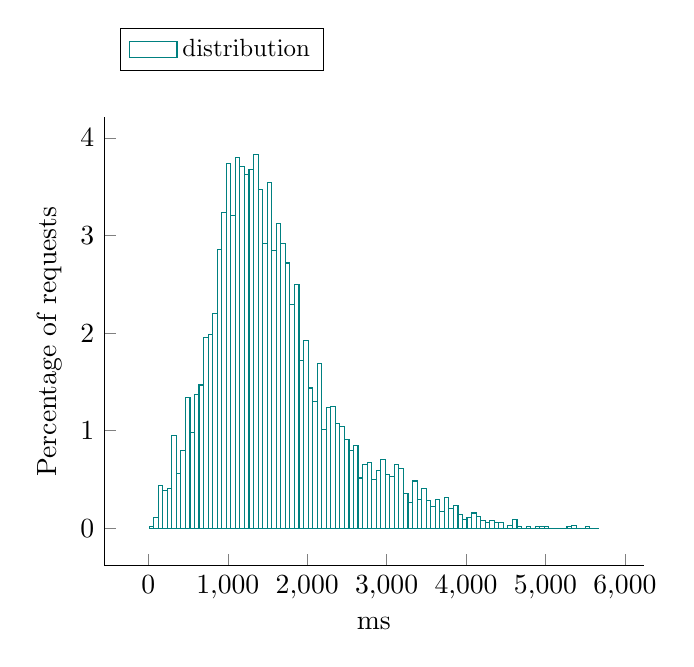
\begin{tikzpicture}
            \begin{axis}[ylabel = Percentage of requests, 
xlabel = ms, 
legend style = {nodes={scale=0.9, transform shape}, at={(0.03,1.2)}, anchor=north west, draw=black, fill=white, align=left, legend columns=3},
area style, mark size = 0pt,
 cycle list name = exotic,
  axis lines* = left]
		\addplot +[ybar interval] coordinates {
			 (9, 0.015625)
			 (66.19, 0.109375)
			 (123.38, 0.4375)
			 (180.57, 0.390625)
			 (237.76, 0.40625)
			 (294.95, 0.953125)
			 (352.14, 0.5625)
			 (409.33, 0.796875)
			 (466.52, 1.34375)
			 (523.71, 0.984375)
			 (580.9, 1.375)
			 (638.09, 1.46875)
			 (695.28, 1.95312)
			 (752.47, 1.98438)
			 (809.66, 2.20312)
			 (866.85, 2.85938)
			 (924.04, 3.23437)
			 (981.23, 3.73438)
			 (1038.42, 3.20312)
			 (1095.61, 3.79688)
			 (1152.8, 3.70312)
			 (1209.99, 3.625)
			 (1267.18, 3.67188)
			 (1324.37, 3.82813)
			 (1381.56, 3.46875)
			 (1438.75, 2.92188)
			 (1495.94, 3.54688)
			 (1553.13, 2.84375)
			 (1610.32, 3.125)
			 (1667.51, 2.92188)
			 (1724.7, 2.71875)
			 (1781.89, 2.29688)
			 (1839.08, 2.5)
			 (1896.27, 1.71875)
			 (1953.46, 1.92188)
			 (2010.65, 1.4375)
			 (2067.84, 1.29688)
			 (2125.03, 1.6875)
			 (2182.22, 1.01562)
			 (2239.41, 1.23438)
			 (2296.6, 1.25)
			 (2353.79, 1.07812)
			 (2410.98, 1.04688)
			 (2468.17, 0.90625)
			 (2525.36, 0.796875)
			 (2582.55, 0.84375)
			 (2639.74, 0.515625)
			 (2696.93, 0.65625)
			 (2754.12, 0.671875)
			 (2811.31, 0.5)
			 (2868.5, 0.59375)
			 (2925.69, 0.703125)
			 (2982.88, 0.546875)
			 (3040.07, 0.53125)
			 (3097.26, 0.65625)
			 (3154.45, 0.609375)
			 (3211.64, 0.359375)
			 (3268.83, 0.265625)
			 (3326.02, 0.484375)
			 (3383.21, 0.296875)
			 (3440.4, 0.40625)
			 (3497.59, 0.28125)
			 (3554.78, 0.21875)
			 (3611.97, 0.296875)
			 (3669.16, 0.171875)
			 (3726.35, 0.3125)
			 (3783.54, 0.203125)
			 (3840.73, 0.234375)
			 (3897.92, 0.140625)
			 (3955.11, 0.09375)
			 (4012.3, 0.109375)
			 (4069.49, 0.15625)
			 (4126.68, 0.125)
			 (4183.87, 0.078125)
			 (4241.06, 0.0625)
			 (4298.25, 0.078125)
			 (4355.44, 0.0625)
			 (4412.63, 0.0625)
			 (4469.82, 0)
			 (4527.01, 0.03125)
			 (4584.2, 0.09375)
			 (4641.39, 0.015625)
			 (4698.58, 0)
			 (4755.77, 0.015625)
			 (4812.96, 0)
			 (4870.15, 0.015625)
			 (4927.34, 0.015625)
			 (4984.53, 0.015625)
			 (5041.72, 0)
			 (5098.91, 0)
			 (5156.1, 0)
			 (5213.29, 0)
			 (5270.48, 0.015625)
			 (5327.67, 0.03125)
			 (5384.86, 0)
			 (5442.05, 0)
			 (5499.24, 0.015625)
			 (5556.43, 0)
			 (5613.62, 0)
			 (5670.81, 0.015625)
		};
\addlegendentry{distribution};
           \end{axis}
      \end{tikzpicture}
  \end{adjustbox}
  \caption{Response time distribution - req = ReadTimeline-0}
\end{figure}
\end{minipage}\hfill\begin{minipage}{0.18\linewidth}
\begin{table}[h]
\begin{tabular}{|cc|}
\hline
\textbf{} & \textbf{ms}\\ \hline
 \Xhline{0.005\arrayrulewidth}
min & 9\\
 \Xhline{0.005\arrayrulewidth}
max & 5728\\
 \Xhline{0.005\arrayrulewidth}
mean & 1590\\
 \Xhline{0.005\arrayrulewidth}
std & 800\\
\hline
\hline
 \Xhline{0.005\arrayrulewidth}
25th & 1041\\
 \Xhline{0.005\arrayrulewidth}
50th & 1437\\
 \Xhline{0.005\arrayrulewidth}
75th & 1963\\
 \Xhline{0.005\arrayrulewidth}
80th & 2147\\
 \Xhline{0.005\arrayrulewidth}
85th & 2382\\
 \Xhline{0.005\arrayrulewidth}
90th & 2714\\
 \Xhline{0.005\arrayrulewidth}
95th & 3189\\
 \Xhline{0.005\arrayrulewidth}
99th & 4034\\
\hline
\end{tabular}
\caption{Response time}
\end{table}
\end{minipage}\hfill